% ============================================================================
% IRC 22:2015 — LIMIT STATE BRIDGE DESIGN VALIDATION FLOWCHART
% Professional Engineering Publication-Ready Document
% ============================================================================
\documentclass[12pt,a4paper]{article}

% ---- Packages ----
\usepackage[utf8]{inputenc}
\usepackage[T1]{fontenc}
\usepackage{lmodern}
\usepackage[top=1.8cm,bottom=1.8cm,left=1.5cm,right=1.5cm]{geometry}
\usepackage{tikz}
\usepackage{amsmath,amssymb}
\usepackage{setspace}
\usepackage{fancyhdr}
\usepackage{xcolor}
\usepackage{booktabs}
\usepackage{tabularx}
\usepackage{enumitem}
\usepackage{float}
\usepackage{caption}
\usepackage[colorlinks=true,linkcolor=blue!60!black,citecolor=green!50!black,urlcolor=blue!70!black]{hyperref}
\usepackage{parskip}

% ---- TikZ Libraries ----
\usetikzlibrary{
  shapes.geometric,
  shapes.symbols,
  arrows.meta,
  positioning,
  calc,
  fit,
  backgrounds,
  decorations.pathreplacing,
  shadows.blur
}

% ---- Colour Palette ----
\definecolor{loadblue}{HTML}{1565C0}
\definecolor{actionteal}{HTML}{00695C}
\definecolor{ulspurple}{HTML}{6A1B9A}
\definecolor{slsorange}{HTML}{E65100}
\definecolor{fatiguerose}{HTML}{AD1457}
\definecolor{dcrgold}{HTML}{F57F17}
\definecolor{passgreen}{HTML}{2E7D32}
\definecolor{failred}{HTML}{C62828}
\definecolor{bglight}{HTML}{F5F5F5}
\definecolor{titledark}{HTML}{1A237E}
\definecolor{subtlegray}{HTML}{757575}

% ---- Page Setup ----
\pagestyle{fancy}
\fancyhf{}
\fancyhead[L]{\small\textcolor{subtlegray}{IRC 22:2015 --- Limit State Design Validation}}
\fancyhead[R]{\small\textcolor{subtlegray}{Karn Agarwal $\cdot$ 2301296}}
\fancyfoot[C]{\thepage}
\renewcommand{\headrulewidth}{0.4pt}
\renewcommand{\footrulewidth}{0.2pt}

\begin{document}

% ============================================================================
%                           TITLE BLOCK
% ============================================================================
\begin{center}
\vspace*{0.3cm}
{\Huge\bfseries\textcolor{titledark}{IRC 22:2015 Validation Flowchart}}\\[0.35cm]
{\Large\textcolor{subtlegray}{Limit State Design Checks for Composite Steel-Concrete Bridge Construction}}\\[0.5cm]
\rule{0.85\textwidth}{1.2pt}\\[0.3cm]
{\normalsize
\textbf{Author:} Karn Agarwal (2301296) \quad
\textbf{Department:} Civil Engineering, Dayalbagh Educational Institute, Agra\\[0.15cm]
\textbf{Standard:} IRC:22-2015 (Third Revision) \quad
\textbf{Reference Loading Code:} IRC:6-2014}\\[0.2cm]
\rule{0.85\textwidth}{0.4pt}
\end{center}

\vspace{0.4cm}

% ============================================================================
%                       MAIN FLOWCHART (Full-Page)
% ============================================================================

\begin{figure}[H]
\centering
\resizebox{\textwidth}{!}{%
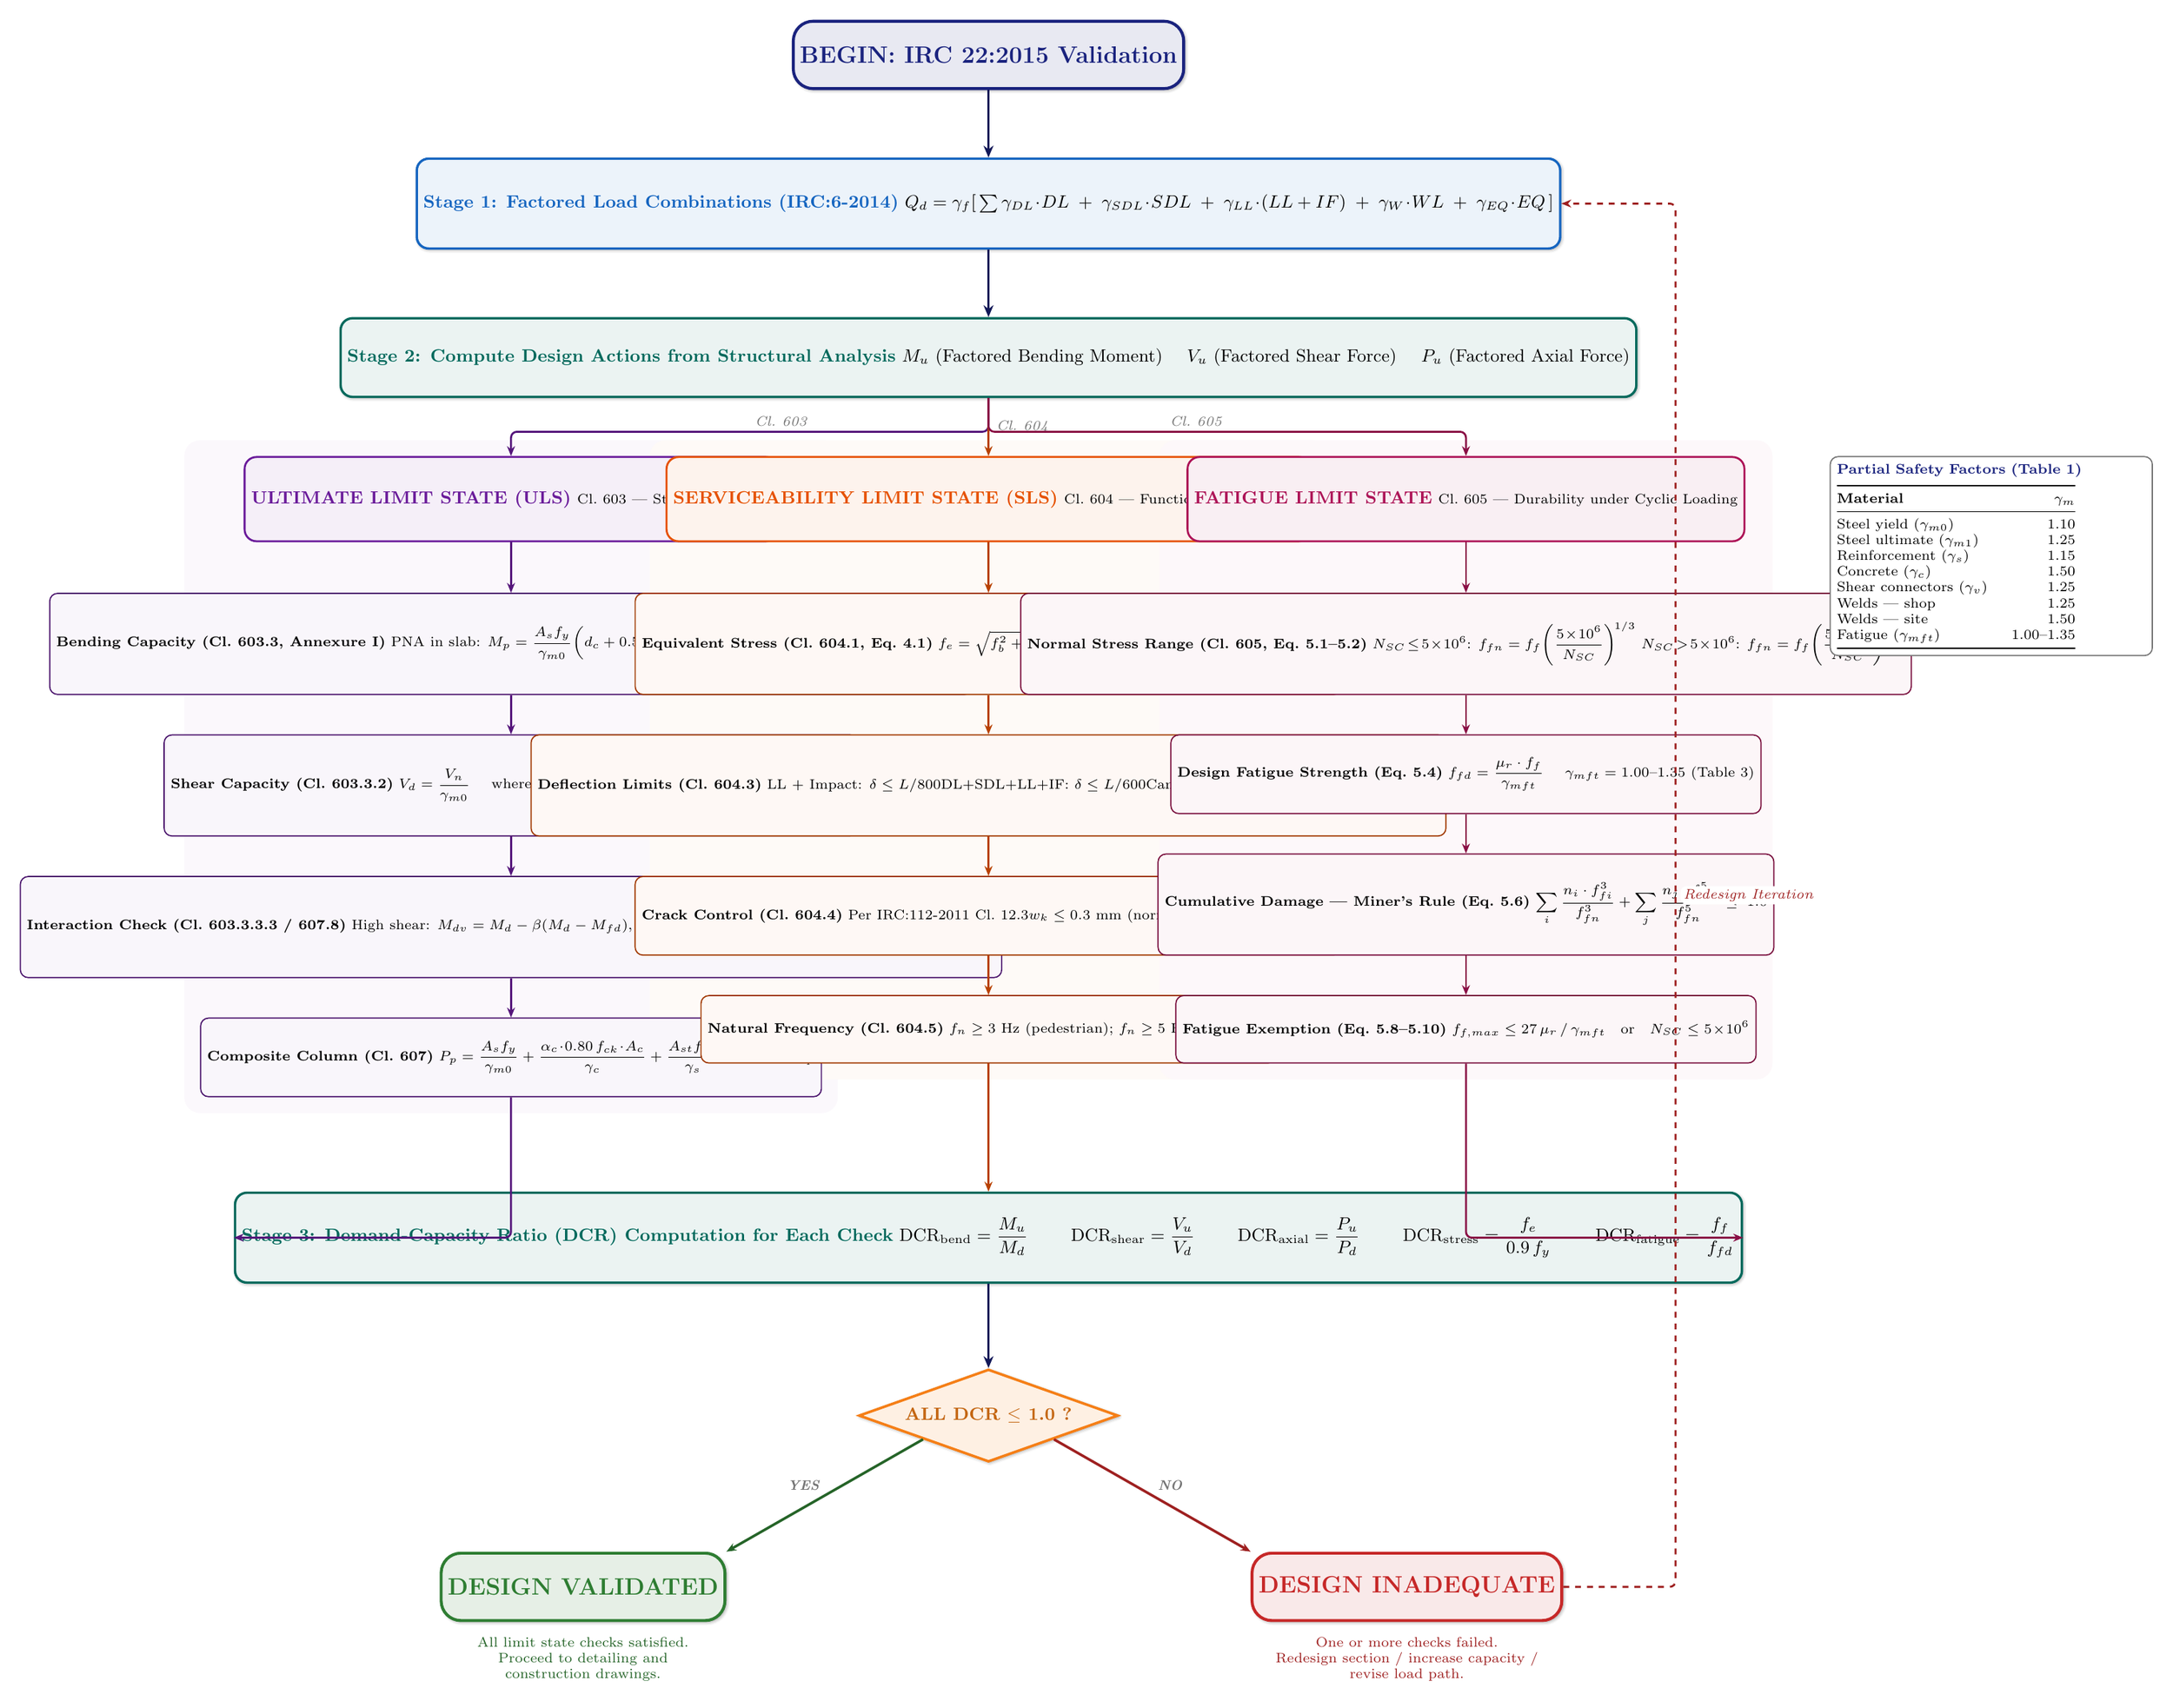
\begin{tikzpicture}[
    % ---- NODE STYLES ----
    startstop/.style={
        rectangle, rounded corners=10pt,
        minimum width=5.5cm, minimum height=1.2cm,
        text centered, font=\bfseries\large,
        draw=titledark, line width=1.5pt,
        fill=titledark!10,
        blur shadow={shadow blur steps=5, shadow xshift=0.8pt, shadow yshift=-0.8pt}
    },
    loadbox/.style={
        rectangle, rounded corners=6pt,
        minimum width=9cm, minimum height=1.6cm,
        text centered, font=\small,
        draw=loadblue, line width=1.2pt,
        fill=loadblue!8,
        blur shadow={shadow blur steps=4, shadow xshift=0.6pt, shadow yshift=-0.6pt}
    },
    actionbox/.style={
        rectangle, rounded corners=6pt,
        minimum width=8cm, minimum height=1.4cm,
        text centered, font=\small,
        draw=actionteal, line width=1.2pt,
        fill=actionteal!8,
        blur shadow={shadow blur steps=4, shadow xshift=0.6pt, shadow yshift=-0.6pt}
    },
    ulsbox/.style={
        rectangle, rounded corners=6pt,
        minimum width=7.8cm, minimum height=1.2cm,
        text centered, font=\small,
        draw=ulspurple, line width=1pt,
        fill=ulspurple!7
    },
    slsbox/.style={
        rectangle, rounded corners=6pt,
        minimum width=7.8cm, minimum height=1.2cm,
        text centered, font=\small,
        draw=slsorange, line width=1pt,
        fill=slsorange!7
    },
    fatbox/.style={
        rectangle, rounded corners=6pt,
        minimum width=7.8cm, minimum height=1.2cm,
        text centered, font=\small,
        draw=fatiguerose, line width=1pt,
        fill=fatiguerose!7
    },
    dcrbox/.style={
        diamond, aspect=2.8,
        minimum width=4cm,
        text centered, font=\small\bfseries,
        draw=dcrgold, line width=1.3pt,
        fill=dcrgold!12,
        blur shadow={shadow blur steps=4, shadow xshift=0.6pt, shadow yshift=-0.6pt}
    },
    passbox/.style={
        rectangle, rounded corners=10pt,
        minimum width=5cm, minimum height=1.2cm,
        text centered, font=\bfseries\large,
        draw=passgreen, line width=1.5pt,
        fill=passgreen!12,
        blur shadow={shadow blur steps=5, shadow xshift=0.8pt, shadow yshift=-0.8pt}
    },
    failbox/.style={
        rectangle, rounded corners=10pt,
        minimum width=5cm, minimum height=1.2cm,
        text centered, font=\bfseries\large,
        draw=failred, line width=1.5pt,
        fill=failred!10,
        blur shadow={shadow blur steps=5, shadow xshift=0.8pt, shadow yshift=-0.8pt}
    },
    formulabox/.style={
        rectangle, rounded corners=4pt,
        minimum width=7.4cm, minimum height=0.9cm,
        text centered, font=\scriptsize,
        draw=#1!70!black, line width=0.6pt,
        fill=#1!4
    },
    branchline/.style={
        ->,
        >={Stealth[length=5pt,width=4pt]},
        line width=1pt,
        color=#1!80!black,
        rounded corners=3pt
    },
    mainline/.style={
        ->,
        >={Stealth[length=6pt,width=5pt]},
        line width=1.2pt,
        color=titledark!70!black,
        rounded corners=3pt
    },
    labelstyle/.style={
        font=\scriptsize\itshape,
        text=subtlegray,
        fill=white,
        inner sep=1.5pt
    }
]

% ==============================
% ROW 0 — START
% ==============================
\node[startstop] (start)
    {\textcolor{titledark}{BEGIN: IRC 22:2015 Validation}};

% ==============================
% ROW 1 — LOAD COMBINATIONS
% ==============================
\node[loadbox, below=1.2cm of start] (loads) {
    \textbf{\textcolor{loadblue}{Stage 1: Factored Load Combinations (IRC:6-2014)}}\\[3pt]
    $Q_d = \gamma_f\!\left[\,\sum\gamma_{DL}\!\cdot\!DL
    \;+\;\gamma_{SDL}\!\cdot\!SDL
    \;+\;\gamma_{LL}\!\cdot\!(LL+IF)
    \;+\;\gamma_W\!\cdot\!WL
    \;+\;\gamma_{EQ}\!\cdot\!EQ\,\right]$
};

% ==============================
% ROW 2 — DESIGN ACTIONS
% ==============================
\node[actionbox, below=1.2cm of loads] (actions) {
    \textbf{\textcolor{actionteal}{Stage 2: Compute Design Actions from Structural Analysis}}\\[3pt]
    $M_u$ (Factored Bending Moment) \quad
    $V_u$ (Factored Shear Force) \quad
    $P_u$ (Factored Axial Force)
};

% ==============================
% ROW 3 — THREE-WAY SPLIT
% ==============================
% Central anchor
\coordinate[below=1.8cm of actions] (split);

% ULS Branch (left)
\node[ulsbox, minimum height=1.5cm] (uls_head) at ([xshift=-8.5cm]split) {
    \textbf{\textcolor{ulspurple}{ULTIMATE LIMIT STATE (ULS)}}\\[2pt]
    {\scriptsize Cl.\ 603 --- Structural Safety}
};

% SLS Branch (centre)
\node[slsbox, minimum height=1.5cm] (sls_head) at (split) {
    \textbf{\textcolor{slsorange}{SERVICEABILITY LIMIT STATE (SLS)}}\\[2pt]
    {\scriptsize Cl.\ 604 --- Functional Performance}
};

% Fatigue Branch (right)
\node[fatbox, minimum height=1.5cm] (fat_head) at ([xshift=8.5cm]split) {
    \textbf{\textcolor{fatiguerose}{FATIGUE LIMIT STATE}}\\[2pt]
    {\scriptsize Cl.\ 605 --- Durability under Cyclic Loading}
};

% ==============================
% ULS SUB-CHECKS
% ==============================
% — Bending Check
\node[formulabox=ulspurple, below=0.9cm of uls_head, minimum height=1.8cm, minimum width=7.8cm] (uls_bend) {
    \textbf{Bending Capacity (Cl.\ 603.3, Annexure~I)}\\[2pt]
    PNA in slab: $M_p = \dfrac{A_s f_y}{\gamma_{m0}}\!\left(d_c + 0.5\,d_s - \dfrac{\lambda x_u}{2}\right)$\\[3pt]
    $x_u = \dfrac{\alpha_{cc}\cdot A_s \cdot f_y}{0.36\,f_{ck}\cdot b_{eff}}$
    \quad $\gamma_{m0}=1.10$
};

% — Shear Check
\node[formulabox=ulspurple, below=0.7cm of uls_bend, minimum height=1.8cm, minimum width=7.8cm] (uls_shear) {
    \textbf{Shear Capacity (Cl.\ 603.3.2)}\\[2pt]
    $V_d = \dfrac{V_n}{\gamma_{m0}}$ \quad where \quad
    $V_p = \dfrac{A_v \cdot f_{yw}}{\sqrt{3}}$\\[3pt]
    Buckling: $\lambda_w = \sqrt{\dfrac{f_{yw}}{\sqrt{3}\;\tau_{cr,e}}}$
};

% — Combined / Interaction
\node[formulabox=ulspurple, below=0.7cm of uls_shear, minimum height=1.8cm, minimum width=7.8cm] (uls_comb) {
    \textbf{Interaction Check (Cl.\ 603.3.3.3 / 607.8)}\\[2pt]
    High shear: $M_{dv} = M_d - \beta(M_d - M_{fd})$, $\beta=(2V/V_d -1)^2$\\[3pt]
    Biaxial: $\dfrac{M_x}{\mu_x M_{px}} + \dfrac{M_y}{\mu_y M_{py}} \leq 1.0$
};

% — Composite Column (if applicable)
\node[formulabox=ulspurple, below=0.7cm of uls_comb, minimum height=1.4cm, minimum width=7.8cm] (uls_col) {
    \textbf{Composite Column (Cl.\ 607)}\\[2pt]
    $P_p = \dfrac{A_s f_y}{\gamma_{m0}} + \dfrac{\alpha_c\!\cdot\!0.80\,f_{ck}\!\cdot\!A_c}{\gamma_c} + \dfrac{A_{st} f_{yk}}{\gamma_s}$
    \quad $P_d = \chi\!\cdot\!P_p$
};

% ==============================
% SLS SUB-CHECKS
% ==============================
% — Stress Check
\node[formulabox=slsorange, below=0.9cm of sls_head, minimum height=1.8cm, minimum width=7.8cm] (sls_stress) {
    \textbf{Equivalent Stress (Cl.\ 604.1, Eq.\ 4.1)}\\[2pt]
    $f_e = \sqrt{f_b^2 + f_b f_p + f_p^2 + 3\tau_b^2} \;\leq\; 0.9\,f_y$\\[3pt]
    {\scriptsize $\gamma_m = 1.00$ at SLS}
};

% — Deflection Check
\node[formulabox=slsorange, below=0.7cm of sls_stress, minimum height=1.8cm, minimum width=7.8cm] (sls_defl) {
    \textbf{Deflection Limits (Cl.\ 604.3)}\\[2pt]
    LL + Impact: $\delta \leq L/800$\\
    DL+SDL+LL+IF: $\delta \leq L/600$\\
    Cantilever: $\delta \leq L/300$ (total), $L/400$ (LL)
};

% — Crack Width
\node[formulabox=slsorange, below=0.7cm of sls_defl, minimum height=1.4cm, minimum width=7.8cm] (sls_crack) {
    \textbf{Crack Control (Cl.\ 604.4)}\\[2pt]
    Per IRC:112-2011 Cl.\ 12.3\\
    $w_k \leq 0.3$~mm (normal), $0.2$~mm (aggressive)
};

% — Vibration
\node[formulabox=slsorange, below=0.7cm of sls_crack, minimum height=1.2cm, minimum width=7.8cm] (sls_vib) {
    \textbf{Natural Frequency (Cl.\ 604.5)}\\[2pt]
    $f_n \geq 3$~Hz (pedestrian); $f_n \geq 5$~Hz (vehicular)
};

% ==============================
% FATIGUE SUB-CHECKS
% ==============================
% — Normal Stress Fatigue
\node[formulabox=fatiguerose, below=0.9cm of fat_head, minimum height=1.8cm, minimum width=7.8cm] (fat_norm) {
    \textbf{Normal Stress Range (Cl.\ 605, Eq.\ 5.1--5.2)}\\[2pt]
    $N_{SC}\!\leq\!5\!\times\!10^6$: $f_{fn} = f_f\!\left(\dfrac{5\!\times\!10^6}{N_{SC}}\right)^{\!1/3}$\\[4pt]
    $N_{SC}\!>\!5\!\times\!10^6$: $f_{fn} = f_f\!\left(\dfrac{5\!\times\!10^6}{N_{SC}}\right)^{\!1/5}$
};

% — Design Fatigue Strength
\node[formulabox=fatiguerose, below=0.7cm of fat_norm, minimum height=1.4cm, minimum width=7.8cm] (fat_design) {
    \textbf{Design Fatigue Strength (Eq.\ 5.4)}\\[2pt]
    $f_{fd} = \dfrac{\mu_r \cdot f_f}{\gamma_{mft}}$
    \quad $\gamma_{mft} = 1.00$--$1.35$ (Table~3)
};

% — Miner's Rule
\node[formulabox=fatiguerose, below=0.7cm of fat_design, minimum height=1.8cm, minimum width=7.8cm] (fat_miner) {
    \textbf{Cumulative Damage --- Miner's Rule (Eq.\ 5.6)}\\[2pt]
    $\displaystyle\sum_{i} \frac{n_i \cdot f_{fi}^3}{f_{fn}^3} + \sum_{j} \frac{n_j \cdot f_{fj}^5}{f_{fn}^5} \;\leq\; 1.0$
};

% — Exemption
\node[formulabox=fatiguerose, below=0.7cm of fat_miner, minimum height=1.2cm, minimum width=7.8cm] (fat_exempt) {
    \textbf{Fatigue Exemption (Eq.\ 5.8--5.10)}\\[2pt]
    $f_{f,max} \leq 27\,\mu_r\,/\,\gamma_{mft}$ \; or \; $N_{SC} \leq 5\!\times\!10^6$
};

% ==============================
% DCR COMPUTATION (BOTTOM MERGE)
% ==============================
\coordinate[below=1cm of uls_col] (uls_bot);
\coordinate[below=1cm of sls_vib] (sls_bot);
\coordinate[below=1cm of fat_exempt] (fat_bot);

% Find the lowest point
\coordinate (merge_y) at ($(sls_bot)+(0,-0.3cm)$);

\node[actionbox, minimum width=14cm, minimum height=1.6cm]
    (dcr_calc) at ([yshift=-1.8cm]merge_y) {
    \textbf{\textcolor{actionteal}{Stage 3: Demand-Capacity Ratio (DCR) Computation for Each Check}}\\[4pt]
    $\text{DCR}_{\text{bend}} = \dfrac{M_u}{M_d}$ \qquad
    $\text{DCR}_{\text{shear}} = \dfrac{V_u}{V_d}$ \qquad
    $\text{DCR}_{\text{axial}} = \dfrac{P_u}{P_d}$ \qquad
    $\text{DCR}_{\text{stress}} = \dfrac{f_e}{0.9\,f_y}$ \qquad
    $\text{DCR}_{\text{fatigue}} = \dfrac{f_f}{f_{fd}}$
};

% ==============================
% DECISION DIAMOND
% ==============================
\node[dcrbox, below=1.5cm of dcr_calc] (decision) {
    \textcolor{dcrgold!80!black}{ALL}\\[2pt]
    \textcolor{dcrgold!80!black}{DCR $\leq$ 1.0 ?}
};

% ==============================
% FINAL OUTCOMES
% ==============================
\node[passbox, below left=2cm and 3.5cm of decision] (pass) {
    \textcolor{passgreen}{DESIGN VALIDATED}
};

\node[failbox, below right=2cm and 3.5cm of decision] (fail) {
    \textcolor{failred}{DESIGN INADEQUATE}
};

% Sub-labels
\node[below=0.15cm of pass, font=\scriptsize, text=passgreen!80!black, text width=5cm, align=center] {
    All limit state checks satisfied.\\
    Proceed to detailing and\\
    construction drawings.
};

\node[below=0.15cm of fail, font=\scriptsize, text=failred!80!black, text width=5cm, align=center] {
    One or more checks failed.\\
    Redesign section / increase capacity /\\
    revise load path.
};

% ==============================
% ARROWS — Main Spine
% ==============================
\draw[mainline] (start) -- (loads);
\draw[mainline] (loads) -- (actions);

% Split arrows
\draw[branchline=ulspurple] (actions.south) -- ++(0,-0.6cm) -| (uls_head.north)
    node[pos=0.25, labelstyle, above right=1pt]{Cl.\ 603};
\draw[branchline=slsorange] (actions.south) -- (sls_head.north)
    node[pos=0.5, labelstyle, right=2pt]{Cl.\ 604};
\draw[branchline=fatiguerose] (actions.south) -- ++(0,-0.6cm) -| (fat_head.north)
    node[pos=0.25, labelstyle, above left=1pt]{Cl.\ 605};

% ULS internal
\draw[branchline=ulspurple] (uls_head) -- (uls_bend);
\draw[branchline=ulspurple] (uls_bend) -- (uls_shear);
\draw[branchline=ulspurple] (uls_shear) -- (uls_comb);
\draw[branchline=ulspurple] (uls_comb) -- (uls_col);

% SLS internal
\draw[branchline=slsorange] (sls_head) -- (sls_stress);
\draw[branchline=slsorange] (sls_stress) -- (sls_defl);
\draw[branchline=slsorange] (sls_defl) -- (sls_crack);
\draw[branchline=slsorange] (sls_crack) -- (sls_vib);

% Fatigue internal
\draw[branchline=fatiguerose] (fat_head) -- (fat_norm);
\draw[branchline=fatiguerose] (fat_norm) -- (fat_design);
\draw[branchline=fatiguerose] (fat_design) -- (fat_miner);
\draw[branchline=fatiguerose] (fat_miner) -- (fat_exempt);

% Merge to DCR
\draw[branchline=ulspurple] (uls_col.south) |- (dcr_calc.west);
\draw[branchline=slsorange]  (sls_vib.south) -- (dcr_calc.north);
\draw[branchline=fatiguerose] (fat_exempt.south) |- (dcr_calc.east);

% DCR to Decision
\draw[mainline] (dcr_calc) -- (decision);

% Decision to outcomes
\draw[branchline=passgreen, line width=1.3pt]
    (decision.south west) -- (pass.north east)
    node[pos=0.5, labelstyle, above left=1pt]{\textbf{YES}};
\draw[branchline=failred, line width=1.3pt]
    (decision.south east) -- (fail.north west)
    node[pos=0.5, labelstyle, above right=1pt]{\textbf{NO}};

% Redesign feedback loop
\draw[branchline=failred, line width=1pt, dashed]
    (fail.east) -- ++(2,0) |- (loads.east)
    node[pos=0.25, labelstyle, right=2pt, text=failred!80!black]{Redesign Iteration};

% ==============================
% BACKGROUND REGIONS
% ==============================
\begin{scope}[on background layer]
\node[fit=(uls_head)(uls_col), fill=ulspurple!3, inner sep=8pt, rounded corners=8pt] {};
\node[fit=(sls_head)(sls_vib), fill=slsorange!3, inner sep=8pt, rounded corners=8pt] {};
\node[fit=(fat_head)(fat_exempt), fill=fatiguerose!3, inner sep=8pt, rounded corners=8pt] {};
\end{scope}

% ==============================
% PARTIAL SAFETY FACTOR TABLE (Side annotation)
% ==============================
\node[draw=subtlegray, rounded corners=4pt, fill=white, line width=0.6pt,
      text width=5.5cm, font=\scriptsize, align=left,
      anchor=north west]
    (psfbox) at ([xshift=1.5cm]fat_head.north east) {
    \textbf{\textcolor{titledark}{Partial Safety Factors (Table~1)}}\\[3pt]
    \begin{tabular}{@{}lr@{}}
    \toprule
    \textbf{Material} & $\gamma_m$ \\
    \midrule
    Steel yield ($\gamma_{m0}$) & 1.10 \\
    Steel ultimate ($\gamma_{m1}$) & 1.25 \\
    Reinforcement ($\gamma_s$) & 1.15 \\
    Concrete ($\gamma_c$) & 1.50 \\
    Shear connectors ($\gamma_v$) & 1.25 \\
    Welds --- shop & 1.25 \\
    Welds --- site & 1.50 \\
    Fatigue ($\gamma_{mft}$) & 1.00--1.35 \\
    \bottomrule
    \end{tabular}
};

\end{tikzpicture}
}% end resizebox
\caption{IRC 22:2015 Limit State Design Validation Flowchart for Composite Steel-Concrete Bridge Construction}
\label{fig:irc22_flowchart}
\end{figure}

\clearpage

% ============================================================================
%               TECHNICAL EXPLANATION
% ============================================================================
\section*{Technical Explanation: Limit State Bridge Design Philosophy under IRC~22:2015}
\addcontentsline{toc}{section}{Technical Explanation}

\subsection*{1.\quad Limit State Design Philosophy}

The limit state method (LSM) is a rational, probabilistic approach to structural design that replaced the older Working Stress Method (WSM) in Indian bridge codes. Instead of applying a single global factor of safety to permissible stresses, LSM considers distinct failure modes --- called \textit{limit states} --- and applies calibrated partial safety factors to loads and material strengths independently.

IRC~22:2015 (Third Revision) requires composite steel-concrete bridge members to be verified against three categories of limit states:

\begin{enumerate}[label=\textbf{(\roman*)}]
    \item \textbf{Ultimate Limit State (ULS) --- Clause~603:} Governs structural safety. The structure must not collapse, overturn, or form a mechanism when subjected to the most adverse factored load combination. ULS checks include bending moment capacity, shear resistance, web buckling, combined bending-shear-axial interaction, and composite column buckling. Material strengths are reduced by partial safety factors ($\gamma_{m0} = 1.10$ for steel yield, $\gamma_c = 1.50$ for concrete) to account for material variability, workmanship, and modelling uncertainty.

    \item \textbf{Serviceability Limit State (SLS) --- Clause~604:} Governs functional performance during normal use. Even if a structure is safe against collapse, it may be unacceptable if it deflects excessively, vibrates uncomfortably, or develops visible cracks. SLS checks use \textit{unfactored} material strengths ($\gamma_m = 1.00$) since the concern is performance rather than survival. The equivalent stress check (Eq.~4.1) limits the combined stress state to $0.9\,f_y$, while deflection limits ($L/800$ for live load, $L/600$ for total) ensure ride quality and structural integrity.

    \item \textbf{Fatigue Limit State --- Clause~605:} Governs durability under repeated cyclic loading. Bridge members experience millions of stress cycles over their design life (typically $2 \times 10^6$ to $10^8$ cycles). Even stress ranges well below the yield strength can cause progressive crack growth at welded joints and stress concentrations. The fatigue check ensures that the applied stress range $f_f$ at any detail category does not exceed the design fatigue strength $f_{fd} = \mu_r f_f / \gamma_{mft}$, where $\mu_r$ is a reliability correction factor and $\gamma_{mft}$ varies from 1.00 (fail-safe, inspectable) to 1.35 (non-fail-safe, non-inspectable) based on consequence and inspection access (Table~3, IRC~22).
\end{enumerate}

The partial safety factor framework separates uncertainty into:
\begin{itemize}
    \item \textbf{Load side:} $\gamma_f$ (load factors from IRC:6-2014) accounts for uncertainty in load magnitude, load modelling, and unfavourable load arrangement.
    \item \textbf{Resistance side:} $\gamma_m$ (material factors from IRC~22, Table~1) accounts for uncertainty in material strength, fabrication tolerances, and analytical model simplification.
\end{itemize}

The structural adequacy condition at any limit state is:

\begin{equation}
\text{Design Action Effect} \;\leq\; \text{Design Resistance}
\end{equation}

or equivalently:

\begin{equation}
\frac{\text{Effect of } \gamma_f \times \text{Characteristic Loads}}{\text{Characteristic Resistance}\,/\,\gamma_m} \;\leq\; 1.0
\end{equation}

\subsection*{2.\quad Role of the Demand-Capacity Ratio (DCR)}

The Demand-Capacity Ratio is a normalised measure of how close a structural member is to its limit state:

\begin{equation}
\text{DCR} = \frac{\text{Demand (Design Action)}}{\text{Capacity (Design Resistance)}}
\end{equation}

\begin{center}
\begin{tabular}{cll}
\toprule
\textbf{DCR Value} & \textbf{Status} & \textbf{Interpretation} \\
\midrule
$\text{DCR} < 0.70$ & Over-designed & Section may be uneconomical; optimise \\
$0.70 \leq \text{DCR} \leq 0.90$ & Efficient & Optimal utilisation with adequate margin \\
$0.90 < \text{DCR} \leq 1.00$ & Adequate & Passes check; limited reserve capacity \\
$\text{DCR} > 1.00$ & \textbf{Fails} & \textbf{Redesign required} \\
\bottomrule
\end{tabular}
\end{center}

For each limit state check in the flowchart, the DCR is computed:

\begin{align}
\text{DCR}_{\text{bending}} &= \frac{M_u}{M_d} & &\text{where } M_d = M_p / \gamma_{m0} \\[4pt]
\text{DCR}_{\text{shear}} &= \frac{V_u}{V_d} & &\text{where } V_d = V_p / \gamma_{m0} \\[4pt]
\text{DCR}_{\text{axial}} &= \frac{P_u}{\chi \cdot P_p} & &\text{(composite column with buckling reduction)} \\[4pt]
\text{DCR}_{\text{stress}} &= \frac{f_e}{0.9\,f_y} & &\text{(SLS equivalent stress)} \\[4pt]
\text{DCR}_{\text{fatigue}} &= \frac{f_f}{f_{fd}} & &\text{(fatigue stress range)}
\end{align}

The design is validated \textit{only when all} DCRs $\leq 1.0$ simultaneously. A single failing DCR renders the entire design inadequate. This is a critical distinction from WSM, where a single global safety factor might mask deficiency in one mode while showing adequacy in another.

\subsection*{3.\quad Safety Margins in IRC~22}

The safety margin is the reserve capacity beyond the design load:

\begin{equation}
\text{Safety Margin} = \frac{1}{\text{DCR}} - 1 = \frac{\text{Capacity} - \text{Demand}}{\text{Demand}}
\end{equation}

For example, a DCR of 0.85 implies a 17.6\% safety margin. Indian bridge codes target an \textit{implicit} reliability level corresponding to a probability of failure $P_f \approx 10^{-5}$ to $10^{-6}$ over the design life (typically 100~years for highway bridges per IRC:6-2014).

The composite safety factor (combining load and material factors) in IRC~22's ULS checks is:

\begin{equation}
\gamma_{\text{composite}} = \gamma_f \times \gamma_m \approx 1.5 \times 1.10 = 1.65 \quad \text{(for steel in bending)}
\end{equation}

This represents an effective factor of safety of 1.65 against the mean strength under the characteristic load --- a significant improvement over WSM's blanket factor of 1.67 applied to permissible stress, because LSM calibrates separate factors for separate uncertainty sources.

\subsection*{4.\quad Structural Reliability Concept}

Structural reliability theory provides the theoretical underpinning for LSM. Consider the \textit{performance function}:

\begin{equation}
g = R - S
\end{equation}

where $R$ is the resistance (capacity) and $S$ is the load effect (demand), both treated as random variables. Failure occurs when $g < 0$. The probability of failure is:

\begin{equation}
P_f = P(g < 0) = P(R < S) = \Phi(-\beta)
\end{equation}

where $\beta$ is the \textbf{reliability index} and $\Phi$ is the standard normal CDF. The relationship between $\beta$ and $P_f$ is:

\begin{center}
\begin{tabular}{ccl}
\toprule
$\beta$ & $P_f$ & \textbf{Application} \\
\midrule
3.1 & $10^{-3}$ & Temporary structures \\
3.8 & $10^{-4}$ & Normal buildings \\
4.3 & $10^{-5}$ & Bridges, dams \\
4.7 & $10^{-6}$ & Nuclear, critical infrastructure \\
\bottomrule
\end{tabular}
\end{center}

IRC~22's partial safety factors have been calibrated (based on Eurocode EN~1990 / EN~1994 lineage) to achieve $\beta \approx 3.8$--$4.3$ for composite bridge members under ULS, corresponding to $P_f \approx 10^{-4}$ to $10^{-5}$ over the reference period. The fatigue partial safety factors ($\gamma_{mft} = 1.00$--$1.35$) are further differentiated by failure consequence (fail-safe vs.\ non-fail-safe) and inspection strategy, reflecting a risk-informed approach.

\subsection*{5.\quad Why IRC Adopts Limit State Design}

India's transition from Working Stress Method to Limit State Method in bridge design codes was driven by several factors:

\begin{enumerate}[label=\textbf{(\alph*)}]
    \item \textbf{Rational safety calibration:} WSM applied a single factor of safety that lumped together all sources of uncertainty. LSM separates load uncertainty ($\gamma_f$) from material uncertainty ($\gamma_m$), permitting more precise calibration. A structure carrying well-defined dead load and uncertain live load is treated differently from one with dominant permanent loads.

    \item \textbf{Consistent reliability:} Under WSM, different structural forms (beams, columns, connections) achieved widely varying reliability levels despite using the same nominal factor of safety. LSM, calibrated through reliability analysis, produces more uniform safety levels across member types.

    \item \textbf{Material efficiency:} By using characteristic strengths (5\% fractile) and applying partial factors, LSM permits higher utilisation of material strength compared to WSM's conservative permissible stresses. Studies show 10--15\% material savings in steel bridge superstructures designed by LSM compared to WSM.

    \item \textbf{Multi-limit-state framework:} WSM only checked stress at working loads. LSM mandates explicit verification at ULS (safety), SLS (performance), and fatigue (durability), ensuring comprehensive structural adequacy.

    \item \textbf{International harmonisation:} IRC~22:2015 is aligned with Eurocode~4 (EN~1994-2) for composite construction, facilitating international collaboration, technology transfer, and design software interoperability. India's growing bridge infrastructure programme (Bharatmala Pariyojana, Setu Bharatam) requires design standards compatible with international practice.

    \item \textbf{Composite construction suitability:} Composite steel-concrete construction exploits the complementary strengths of steel (tension, ductility) and concrete (compression, fire resistance). The nonlinear behaviour of composite sections, including partial shear connection, staged construction effects, and concrete creep/shrinkage, is more accurately captured by the LSM framework than by elastic WSM analysis.

    \item \textbf{Performance-based design path:} LSM provides a natural pathway to performance-based design, where the designer can target specific reliability levels for different consequence classes. This is critical for bridges, where failure consequences (human casualties, traffic disruption, economic loss) are significantly higher than for ordinary buildings.
\end{enumerate}

\vspace{0.5cm}
\begin{center}
\rule{0.6\textwidth}{0.5pt}\\[0.3cm]
{\small\textit{Document prepared in accordance with IRC:22-2015 (Third Revision), IRC:6-2014, and IS~800:2007.\\
For academic and professional reference. Not a substitute for full code compliance by licensed engineers.}}
\end{center}

\end{document}
